\documentclass{standalone}
% This file was created with tikzplotlib v0.9.15.

\usepackage{siunitx}
\usepackage{pgfplots}
% and optionally (as of Pgfplots 1.3):
\pgfplotsset{compat=newest}
\pgfplotsset{plot coordinates/math parser=false}
\newlength\figureheight
\newlength\figurewidth

\newcommand{\Set}[1]{\mathcal{#1}}
\newcommand{\Vector}[1]{\bm{\MakeLowercase{#1}}}
\newcommand{\Operator}[1]{\bm{\MakeUppercase{#1}}}
%%%%%%%%%%
\DeclareMathAlphabet{\mathsfbr}{OT1}{cmss}{m}{n}%for math sans serif (cmss)
\SetMathAlphabet{\mathsfbr}{bold}{OT1}{cmss}{bx}{n}%for math sans serif (cmss)
\DeclareRobustCommand{\msf}[1]{%
  \ifcat\noexpand#1\relax\msfgreek{#1}\else\mathsfbr{#1}\fi%for math sans serif (cmss)
}
\DeclareFontEncoding{LGR}{}{} % or load \usepackage{textgreek}
\DeclareSymbolFont{sfgreek}{LGR}{cmss}{m}{n}
\SetSymbolFont{sfgreek}{bold}{LGR}{cmss}{bx}{n}
\DeclareMathSymbol{\sXi}{\mathalpha}{sfgreek}{`X}
\DeclareMathSymbol{\sUpsilon}{\mathalpha}{sfgreek}{`U}

\begin{document}
% This file was created with tikzplotlib v0.9.15.
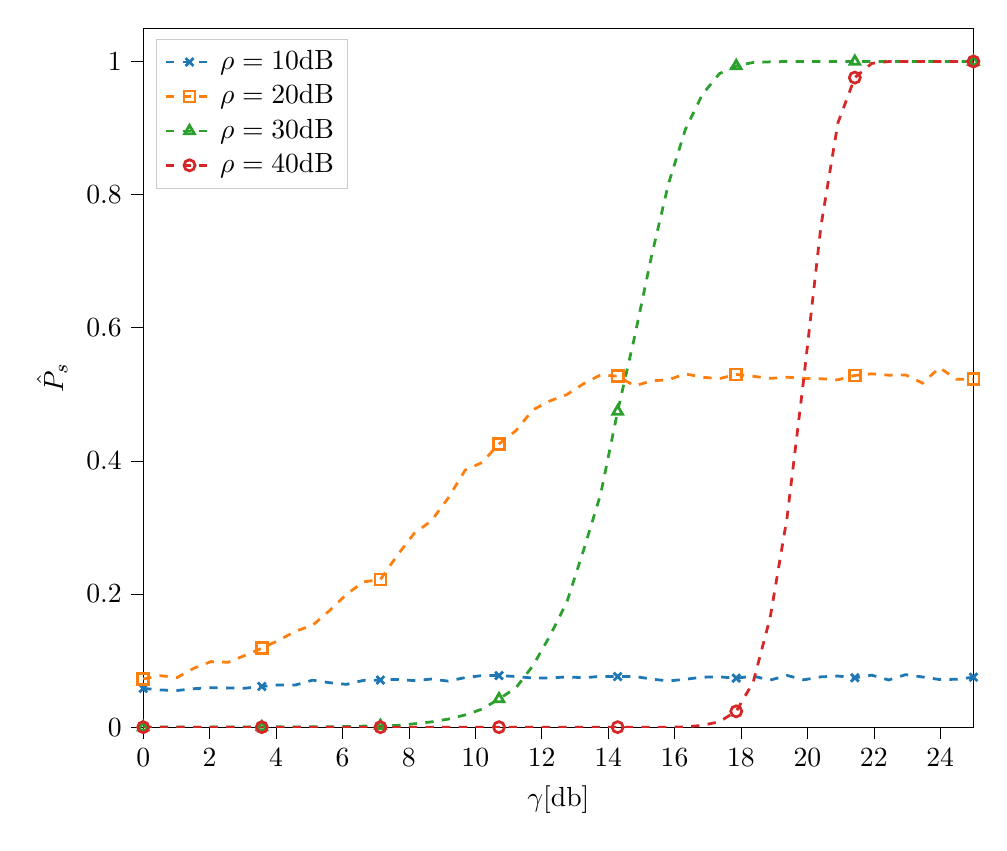
\begin{tikzpicture}

\definecolor{color0}{rgb}{0.12156862745098,0.466666666666667,0.705882352941177}
\definecolor{color1}{rgb}{1,0.498039215686275,0.0549019607843137}
\definecolor{color2}{rgb}{0.172549019607843,0.627450980392157,0.172549019607843}
\definecolor{color3}{rgb}{0.83921568627451,0.152941176470588,0.156862745098039}

\begin{axis}[
width=1\linewidth,
legend cell align={left},
legend style={
  fill opacity=0.8,
  draw opacity=1,
  text opacity=1,
  at={(0.015,0.985)},
  anchor=north west,
  draw=white!80!black
},
tick align=outside,
tick pos=left,
%title={Threshold crossing search},
x grid style={white!69.0196078431373!black},
xlabel={$\gamma [\si{db}]$},
xmin=0, xmax=25,
xtick style={color=black},
y grid style={white!69.0196078431373!black},
ylabel={$\hat{P}_{s}$},
ymin=0, ymax=1.05,
ytick style={color=black}
]
\addplot [dashed, semithick, color0, line width=1pt, mark=x, mark options={solid, color0}, mark repeat=7]
table {%
0 0.0583
0.510204081632653 0.0559
1.02040816326531 0.0551
1.53061224489796 0.0578
2.04081632653061 0.0592
2.55102040816327 0.059
3.06122448979592 0.0585
3.57142857142857 0.0612
4.08163265306122 0.0635
4.59183673469388 0.0635
5.10204081632653 0.0706
5.61224489795918 0.0668
6.12244897959184 0.0643
6.63265306122449 0.0703
7.14285714285714 0.0707
7.6530612244898 0.0718
8.16326530612245 0.0699
8.6734693877551 0.0723
9.18367346938776 0.0692
9.69387755102041 0.0745
10.2040816326531 0.0775
10.7142857142857 0.0775
11.2244897959184 0.0761
11.734693877551 0.0738
12.2448979591837 0.0738
12.7551020408163 0.0756
13.265306122449 0.0742
13.7755102040816 0.0764
14.2857142857143 0.076
14.7959183673469 0.0762
15.3061224489796 0.0723
15.8163265306122 0.0694
16.3265306122449 0.072
16.8367346938776 0.0751
17.3469387755102 0.0756
17.8571428571429 0.0736
18.3673469387755 0.0767
18.8775510204082 0.0707
19.3877551020408 0.0777
19.8979591836735 0.0712
20.4081632653061 0.0756
20.9183673469388 0.0768
21.4285714285714 0.0742
21.9387755102041 0.0781
22.4489795918367 0.0709
22.9591836734694 0.0789
23.469387755102 0.0754
23.9795918367347 0.0716
24.4897959183673 0.0719
25 0.0751
};
\addlegendentry{$\rho = 10 \si{dB}$}
\addplot [dashed, semithick, color1, line width=1pt, mark=square, mark options={solid, color1}, mark repeat=7]
table {%
0 0.0724
0.510204081632653 0.0774
1.02040816326531 0.0745
1.53061224489796 0.0887
2.04081632653061 0.0985
2.55102040816327 0.0975
3.06122448979592 0.1077
3.57142857142857 0.1185
4.08163265306122 0.1306
4.59183673469388 0.1443
5.10204081632653 0.1531
5.61224489795918 0.1752
6.12244897959184 0.1996
6.63265306122449 0.2183
7.14285714285714 0.2218
7.6530612244898 0.2584
8.16326530612245 0.2913
8.6734693877551 0.3098
9.18367346938776 0.3441
9.69387755102041 0.3861
10.2040816326531 0.3976
10.7142857142857 0.4255
11.2244897959184 0.4455
11.734693877551 0.4767
12.2448979591837 0.49
12.7551020408163 0.4996
13.265306122449 0.5161
13.7755102040816 0.5293
14.2857142857143 0.5272
14.7959183673469 0.5127
15.3061224489796 0.5202
15.8163265306122 0.522
16.3265306122449 0.5307
16.8367346938776 0.5257
17.3469387755102 0.5236
17.8571428571429 0.5299
18.3673469387755 0.5271
18.8775510204082 0.524
19.3877551020408 0.5257
19.8979591836735 0.524
20.4081632653061 0.5235
20.9183673469388 0.5218
21.4285714285714 0.5284
21.9387755102041 0.5308
22.4489795918367 0.5288
22.9591836734694 0.5292
23.469387755102 0.5168
23.9795918367347 0.5401
24.4897959183673 0.5226
25 0.5227
};
\addlegendentry{$\rho = 20 \si{dB}$}
\addplot [dashed, semithick, color2, line width=1pt, mark=triangle, mark options={solid, color2}, mark repeat=7]
table {%
0 0
0.510204081632653 0.0001
1.02040816326531 0.0003
1.53061224489796 0
2.04081632653061 0.0001
2.55102040816327 0.0003
3.06122448979592 0.0002
3.57142857142857 0.0002
4.08163265306122 0.0005
4.59183673469388 0.0001
5.10204081632653 0.0007
5.61224489795918 0.0007
6.12244897959184 0.001
6.63265306122449 0.0016
7.14285714285714 0.0022
7.6530612244898 0.0027
8.16326530612245 0.0051
8.6734693877551 0.0079
9.18367346938776 0.0121
9.69387755102041 0.0184
10.2040816326531 0.0271
10.7142857142857 0.0424
11.2244897959184 0.0592
11.734693877551 0.0923
12.2448979591837 0.137
12.7551020408163 0.1876
13.265306122449 0.2667
13.7755102040816 0.3502
14.2857142857143 0.4744
14.7959183673469 0.5863
15.3061224489796 0.7075
15.8163265306122 0.8162
16.3265306122449 0.898
16.8367346938776 0.9504
17.3469387755102 0.9816
17.8571428571429 0.9934
18.3673469387755 0.9985
18.8775510204082 0.9995
19.3877551020408 1
19.8979591836735 0.9998
20.4081632653061 1
20.9183673469388 0.9999
21.4285714285714 1
21.9387755102041 0.9999
22.4489795918367 1
22.9591836734694 0.9998
23.469387755102 1
23.9795918367347 1
24.4897959183673 1
25 0.9998
};
\addlegendentry{$\rho = 30 \si{dB}$}
\addplot [dashed,semithick, color3, line width=1pt, mark=o, mark options={solid, color3}, mark repeat=7]
table {%
0 0
0.510204081632653 0
1.02040816326531 0
1.53061224489796 0
2.04081632653061 0
2.55102040816327 0
3.06122448979592 0
3.57142857142857 0
4.08163265306122 0
4.59183673469388 0
5.10204081632653 0
5.61224489795918 0
6.12244897959184 0
6.63265306122449 0
7.14285714285714 0
7.6530612244898 0
8.16326530612245 0
8.6734693877551 0
9.18367346938776 0
9.69387755102041 0
10.2040816326531 0
10.7142857142857 0
11.2244897959184 0
11.734693877551 0
12.2448979591837 0
12.7551020408163 0
13.265306122449 0
13.7755102040816 0
14.2857142857143 0
14.7959183673469 0
15.3061224489796 0
15.8163265306122 0
16.3265306122449 0.0005
16.8367346938776 0.0027
17.3469387755102 0.0081
17.8571428571429 0.0238
18.3673469387755 0.0676
18.8775510204082 0.1642
19.3877551020408 0.3147
19.8979591836735 0.5266
20.4081632653061 0.7528
20.9183673469388 0.9077
21.4285714285714 0.9758
21.9387755102041 0.9972
22.4489795918367 0.9999
22.9591836734694 1
23.469387755102 1
23.9795918367347 1
24.4897959183673 1
25 1
};
\addlegendentry{$\rho = 40 \si{dB}$}
\end{axis}

\end{tikzpicture}
\end{document}